\tikzset {_dao9utne7/.code = {\pgfsetadditionalshadetransform{ \pgftransformshift{\pgfpoint{0 bp } { 0 bp }  }  \pgftransformrotate{-117 }  \pgftransformscale{2 }  }}}
\pgfdeclarehorizontalshading{_nakw2h43n}{150bp}{rgb(0bp)=(1,1,1);
    rgb(37.5bp)=(1,1,1);
    rgb(50.08184160505022bp)=(0.95,0.95,0.95);
    rgb(57.64583042689732bp)=(0.88,0.88,0.88);
    rgb(61.33184160505022bp)=(0.96,0.96,0.96);
    rgb(100bp)=(0.96,0.96,0.96)}
\tikzset {_yzwn2ombi/.code = {\pgfsetadditionalshadetransform{ \pgftransformshift{\pgfpoint{0 bp } { 0 bp }  }  \pgftransformrotate{-117 }  \pgftransformscale{2 }  }}}
\pgfdeclarehorizontalshading{_0lmbx59yl}{150bp}{rgb(0bp)=(1,1,1);
    rgb(37.5bp)=(1,1,1);
    rgb(50.08184160505022bp)=(0.95,0.95,0.95);
    rgb(57.64583042689732bp)=(0.88,0.88,0.88);
    rgb(61.33184160505022bp)=(0.96,0.96,0.96);
    rgb(100bp)=(0.96,0.96,0.96)}
\tikzset {_u5d5qei3l/.code = {\pgfsetadditionalshadetransform{ \pgftransformshift{\pgfpoint{0 bp } { 0 bp }  }  \pgftransformrotate{-117 }  \pgftransformscale{2 }  }}}
\pgfdeclarehorizontalshading{_bvfni0dfh}{150bp}{rgb(0bp)=(1,1,1);
    rgb(37.5bp)=(1,1,1);
    rgb(50.08184160505022bp)=(0.95,0.95,0.95);
    rgb(57.64583042689732bp)=(0.88,0.88,0.88);
    rgb(61.33184160505022bp)=(0.96,0.96,0.96);
    rgb(100bp)=(0.96,0.96,0.96)}
\tikzset {_8s69p9fbu/.code = {\pgfsetadditionalshadetransform{ \pgftransformshift{\pgfpoint{0 bp } { 0 bp }  }  \pgftransformrotate{-117 }  \pgftransformscale{2 }  }}}
\pgfdeclarehorizontalshading{_oawzao3ec}{150bp}{rgb(0bp)=(1,1,1);
    rgb(37.5bp)=(1,1,1);
    rgb(50.08184160505022bp)=(0.95,0.95,0.95);
    rgb(57.64583042689732bp)=(0.88,0.88,0.88);
    rgb(61.33184160505022bp)=(0.96,0.96,0.96);
    rgb(100bp)=(0.96,0.96,0.96)}
\tikzset {_u07eqnzna/.code = {\pgfsetadditionalshadetransform{ \pgftransformshift{\pgfpoint{0 bp } { 0 bp }  }  \pgftransformrotate{-117 }  \pgftransformscale{2 }  }}}
\pgfdeclarehorizontalshading{_qjadfddxj}{150bp}{rgb(0bp)=(1,1,1);
    rgb(37.5bp)=(1,1,1);
    rgb(50.08184160505022bp)=(0.95,0.95,0.95);
    rgb(57.64583042689732bp)=(0.88,0.88,0.88);
    rgb(61.33184160505022bp)=(0.96,0.96,0.96);
    rgb(100bp)=(0.96,0.96,0.96)}
\tikzset {_zxlil0jj4/.code = {\pgfsetadditionalshadetransform{ \pgftransformshift{\pgfpoint{0 bp } { 0 bp }  }  \pgftransformrotate{-117 }  \pgftransformscale{2 }  }}}
\pgfdeclarehorizontalshading{_zgf1vcc1n}{150bp}{rgb(0bp)=(1,1,1);
    rgb(37.5bp)=(1,1,1);
    rgb(50.08184160505022bp)=(0.95,0.95,0.95);
    rgb(57.64583042689732bp)=(0.88,0.88,0.88);
    rgb(61.33184160505022bp)=(0.96,0.96,0.96);
    rgb(100bp)=(0.96,0.96,0.96)}
\tikzset {_y8tg49i5q/.code = {\pgfsetadditionalshadetransform{ \pgftransformshift{\pgfpoint{0 bp } { 0 bp }  }  \pgftransformrotate{-117 }  \pgftransformscale{2 }  }}}
\pgfdeclarehorizontalshading{_3r1bynmjn}{150bp}{rgb(0bp)=(1,1,1);
    rgb(37.5bp)=(1,1,1);
    rgb(50.08184160505022bp)=(0.95,0.95,0.95);
    rgb(57.64583042689732bp)=(0.88,0.88,0.88);
    rgb(61.33184160505022bp)=(0.96,0.96,0.96);
    rgb(100bp)=(0.96,0.96,0.96)}
\tikzset {_breusdai9/.code = {\pgfsetadditionalshadetransform{ \pgftransformshift{\pgfpoint{0 bp } { 0 bp }  }  \pgftransformrotate{-76 }  \pgftransformscale{2 }  }}}
\pgfdeclarehorizontalshading{_tnci4tz1g}{150bp}{rgb(0bp)=(0.65,0.81,0.87);
    rgb(37.5bp)=(0.65,0.81,0.87);
    rgb(50.16369138445173bp)=(0.29,0.56,0.89);
    rgb(62.5bp)=(0.29,0.56,0.89);
    rgb(100bp)=(0.29,0.56,0.89)}
\tikzset{_ba6zrqmob/.code = {\pgfsetadditionalshadetransform{\pgftransformshift{\pgfpoint{0 bp } { 0 bp }  }  \pgftransformrotate{-76 }  \pgftransformscale{2 } }}}
\pgfdeclarehorizontalshading{_x4usmzgac} {150bp} {color(0bp)=(transparent!0);
    color(37.5bp)=(transparent!0);
    color(50.16369138445173bp)=(transparent!84);
    color(62.5bp)=(transparent!35);
    color(100bp)=(transparent!35) }
\pgfdeclarefading{_9kkfwoljy}{\tikz \fill[shading=_x4usmzgac,_ba6zrqmob] (0,0) rectangle (50bp,50bp); }
\tikzset{every picture/.style={line width=0.75pt}}
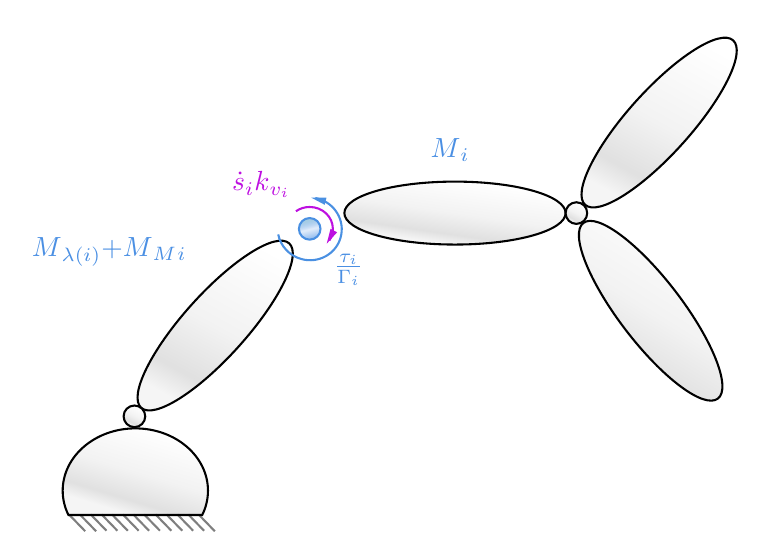
\begin{tikzpicture}[x=0.75pt,y=0.75pt,yscale=-1,xscale=1]
    \path  [shading=_nakw2h43n,_dao9utne7] (169.48,170.37) .. controls (169.48,161.99) and (193.34,155.2) .. (222.77,155.2) .. controls (252.21,155.2) and (276.07,161.99) .. (276.07,170.37) .. controls (276.07,178.74) and (252.21,185.53) .. (222.77,185.53) .. controls (193.34,185.53) and (169.48,178.74) .. (169.48,170.37) -- cycle ;
    \draw  [color={rgb, 255:red, 0; green, 0; blue, 0 }  ,draw opacity=1 ][line width=0.75]  (169.48,170.37) .. controls (169.48,161.99) and (193.34,155.2) .. (222.77,155.2) .. controls (252.21,155.2) and (276.07,161.99) .. (276.07,170.37) .. controls (276.07,178.74) and (252.21,185.53) .. (222.77,185.53) .. controls (193.34,185.53) and (169.48,178.74) .. (169.48,170.37) -- cycle ;
    \path  [shading=_0lmbx59yl,_yzwn2ombi] (356.79,87.15) .. controls (363.01,92.75) and (352.1,115.03) .. (332.41,136.9) .. controls (312.72,158.78) and (291.71,171.97) .. (285.48,166.37) .. controls (279.26,160.76) and (290.17,138.49) .. (309.86,116.61) .. controls (329.55,94.73) and (350.56,81.54) .. (356.79,87.15) -- cycle ;
    \draw  [color={rgb, 255:red, 0; green, 0; blue, 0 }  ,draw opacity=1 ][line width=0.75]  (356.79,87.15) .. controls (363.01,92.75) and (352.1,115.03) .. (332.41,136.9) .. controls (312.72,158.78) and (291.71,171.97) .. (285.48,166.37) .. controls (279.26,160.76) and (290.17,138.49) .. (309.86,116.61) .. controls (329.55,94.73) and (350.56,81.54) .. (356.79,87.15) -- cycle ;
    \path  [shading=_bvfni0dfh,_u5d5qei3l] (276.07,170.37) .. controls (276.07,167.49) and (278.4,165.16) .. (281.27,165.16) .. controls (284.15,165.16) and (286.48,167.49) .. (286.48,170.37) .. controls (286.48,173.24) and (284.15,175.57) .. (281.27,175.57) .. controls (278.4,175.57) and (276.07,173.24) .. (276.07,170.37) -- cycle ;
    \draw  [color={rgb, 255:red, 0; green, 0; blue, 0 }  ,draw opacity=1 ][line width=0.75]  (276.07,170.37) .. controls (276.07,167.49) and (278.4,165.16) .. (281.27,165.16) .. controls (284.15,165.16) and (286.48,167.49) .. (286.48,170.37) .. controls (286.48,173.24) and (284.15,175.57) .. (281.27,175.57) .. controls (278.4,175.57) and (276.07,173.24) .. (276.07,170.37) -- cycle ;
    \path  [shading=_oawzao3ec,_8s69p9fbu] (142.89,184.95) .. controls (149.11,190.55) and (138.2,212.83) .. (118.51,234.7) .. controls (98.82,256.58) and (77.81,269.77) .. (71.58,264.17) .. controls (65.36,258.56) and (76.27,236.29) .. (95.96,214.41) .. controls (115.65,192.53) and (136.66,179.34) .. (142.89,184.95) -- cycle ;
    \draw  [color={rgb, 255:red, 0; green, 0; blue, 0 }  ,draw opacity=1 ][line width=0.75]  (142.89,184.95) .. controls (149.11,190.55) and (138.2,212.83) .. (118.51,234.7) .. controls (98.82,256.58) and (77.81,269.77) .. (71.58,264.17) .. controls (65.36,258.56) and (76.27,236.29) .. (95.96,214.41) .. controls (115.65,192.53) and (136.66,179.34) .. (142.89,184.95) -- cycle ;
    \path  [shading=_qjadfddxj,_u07eqnzna] (63.12,268.29) .. controls (63.12,265.42) and (65.46,263.08) .. (68.33,263.08) .. controls (71.21,263.08) and (73.54,265.42) .. (73.54,268.29) .. controls (73.54,271.17) and (71.21,273.5) .. (68.33,273.5) .. controls (65.46,273.5) and (63.12,271.17) .. (63.12,268.29) -- cycle ;
    \draw  [color={rgb, 255:red, 0; green, 0; blue, 0 }  ,draw opacity=1 ][line width=0.75]  (63.12,268.29) .. controls (63.12,265.42) and (65.46,263.08) .. (68.33,263.08) .. controls (71.21,263.08) and (73.54,265.42) .. (73.54,268.29) .. controls (73.54,271.17) and (71.21,273.5) .. (68.33,273.5) .. controls (65.46,273.5) and (63.12,271.17) .. (63.12,268.29) -- cycle ;
    \path  [shading=_zgf1vcc1n,_zxlil0jj4] (349.45,259.74) .. controls (342.8,264.83) and (322.9,250.01) .. (305.01,226.64) .. controls (287.11,203.27) and (278,180.2) .. (284.65,175.11) .. controls (291.3,170.02) and (311.2,184.83) .. (329.09,208.2) .. controls (346.98,231.57) and (356.1,254.64) .. (349.45,259.74) -- cycle ;
    \draw  [color={rgb, 255:red, 0; green, 0; blue, 0 }  ,draw opacity=1 ][line width=0.75]  (349.45,259.74) .. controls (342.8,264.83) and (322.9,250.01) .. (305.01,226.64) .. controls (287.11,203.27) and (278,180.2) .. (284.65,175.11) .. controls (291.3,170.02) and (311.2,184.83) .. (329.09,208.2) .. controls (346.98,231.57) and (356.1,254.64) .. (349.45,259.74) -- cycle ;
    \path  [shading=_3r1bynmjn,_y8tg49i5q] (36.54,315.83) .. controls (34.76,312.23) and (33.77,308.26) .. (33.77,304.1) .. controls (33.77,287.53) and (49.44,274.1) .. (68.77,274.1) .. controls (88.1,274.1) and (103.77,287.53) .. (103.77,304.1) .. controls (103.77,308.26) and (102.78,312.23) .. (100.99,315.83) -- cycle ;
    \draw   (36.54,315.83) .. controls (34.76,312.23) and (33.77,308.26) .. (33.77,304.1) .. controls (33.77,287.53) and (49.44,274.1) .. (68.77,274.1) .. controls (88.1,274.1) and (103.77,287.53) .. (103.77,304.1) .. controls (103.77,308.26) and (102.78,312.23) .. (100.99,315.83) -- cycle ;
    \draw [color={rgb, 255:red, 0; green, 0; blue, 0 }  ,draw opacity=0.5 ]   (37.04,315.83) -- (44.63,323.66) ;
    \draw [color={rgb, 255:red, 0; green, 0; blue, 0 }  ,draw opacity=0.5 ]   (99.49,315.83) -- (107.07,323.66) ;
    \draw [color={rgb, 255:red, 0; green, 0; blue, 0 }  ,draw opacity=0.5 ]   (42.29,315.83) -- (49.88,323.66) ;
    \draw [color={rgb, 255:red, 0; green, 0; blue, 0 }  ,draw opacity=0.5 ]   (47.29,315.58) -- (54.88,323.41) ;
    \draw [color={rgb, 255:red, 0; green, 0; blue, 0 }  ,draw opacity=0.5 ]   (52.54,315.58) -- (60.13,323.41) ;
    \draw [color={rgb, 255:red, 0; green, 0; blue, 0 }  ,draw opacity=0.5 ]   (57.54,315.58) -- (65.13,323.41) ;
    \draw [color={rgb, 255:red, 0; green, 0; blue, 0 }  ,draw opacity=0.5 ]   (62.79,315.58) -- (70.38,323.41) ;
    \draw [color={rgb, 255:red, 0; green, 0; blue, 0 }  ,draw opacity=0.5 ]   (67.79,315.58) -- (75.38,323.41) ;
    \draw [color={rgb, 255:red, 0; green, 0; blue, 0 }  ,draw opacity=0.5 ]   (73.04,315.58) -- (80.63,323.41) ;
    \draw [color={rgb, 255:red, 0; green, 0; blue, 0 }  ,draw opacity=0.5 ]   (78.54,315.58) -- (86.13,323.41) ;
    \draw [color={rgb, 255:red, 0; green, 0; blue, 0 }  ,draw opacity=0.5 ]   (83.79,315.58) -- (91.38,323.41) ;
    \draw [color={rgb, 255:red, 0; green, 0; blue, 0 }  ,draw opacity=0.5 ]   (89.04,315.58) -- (96.63,323.41) ;
    \draw [color={rgb, 255:red, 0; green, 0; blue, 0 }  ,draw opacity=0.5 ]   (94.29,315.58) -- (101.88,323.41) ;
    \path  [shading=_tnci4tz1g,_breusdai9,path fading= _9kkfwoljy ,fading transform={xshift=2}] (147.57,177.97) .. controls (147.57,175.09) and (149.9,172.76) .. (152.77,172.76) .. controls (155.65,172.76) and (157.98,175.09) .. (157.98,177.97) .. controls (157.98,180.84) and (155.65,183.17) .. (152.77,183.17) .. controls (149.9,183.17) and (147.57,180.84) .. (147.57,177.97) -- cycle ;
    \draw  [color={rgb, 255:red, 74; green, 144; blue, 226 }  ,draw opacity=1 ][line width=0.75]  (147.57,177.97) .. controls (147.57,175.09) and (149.9,172.76) .. (152.77,172.76) .. controls (155.65,172.76) and (157.98,175.09) .. (157.98,177.97) .. controls (157.98,180.84) and (155.65,183.17) .. (152.77,183.17) .. controls (149.9,183.17) and (147.57,180.84) .. (147.57,177.97) -- cycle ;
    \draw  [draw opacity=0] (146.14,169.49) .. controls (147.99,168.19) and (150.29,167.42) .. (152.77,167.42) .. controls (158.94,167.42) and (163.94,172.14) .. (163.94,177.97) .. controls (163.94,180.72) and (162.82,183.23) .. (160.99,185.11) -- (152.77,177.97) -- cycle ; \draw [color={rgb, 255:red, 189; green, 16; blue, 224 }  ,draw opacity=1 ]   (146.14,169.49) .. controls (147.99,168.19) and (150.29,167.42) .. (152.77,167.42) .. controls (158.94,167.42) and (163.94,172.14) .. (163.94,177.97) .. controls (163.94,180.03) and (163.31,181.96) .. (162.22,183.59) ; \draw [shift={(160.99,185.11)}, rotate = 298.36] [fill={rgb, 255:red, 189; green, 16; blue, 224 }  ,fill opacity=1 ][line width=0.08]  [draw opacity=0] (7.2,-1.8) -- (0,0) -- (7.2,1.8) -- cycle    ;
    \draw  [draw opacity=0] (153.45,162.87) .. controls (154.53,162.93) and (155.62,163.11) .. (156.7,163.4) .. controls (164.95,165.62) and (169.88,173.95) .. (167.71,181.99) .. controls (165.55,190.04) and (157.1,194.76) .. (148.85,192.53) .. controls (142.92,190.94) and (138.71,186.19) .. (137.61,180.66) -- (152.77,177.97) -- cycle ; \draw [color={rgb, 255:red, 74; green, 144; blue, 226 }  ,draw opacity=1 ]   (155.45,163.11) .. controls (155.87,163.19) and (156.29,163.29) .. (156.7,163.4) .. controls (164.95,165.62) and (169.88,173.95) .. (167.71,181.99) .. controls (165.55,190.04) and (157.1,194.76) .. (148.85,192.53) .. controls (142.92,190.94) and (138.71,186.19) .. (137.61,180.66) ;  \draw [shift={(153.45,162.87)}, rotate = 14.08] [fill={rgb, 255:red, 74; green, 144; blue, 226 }  ,fill opacity=1 ][line width=0.08]  [draw opacity=0] (7.2,-1.8) -- (0,0) -- (7.2,1.8) -- cycle    ;
    \draw (17.4,180.6) node [anchor=north west][inner sep=0.75pt]    {$\textcolor[rgb]{0.29,0.56,0.89}{M}\textcolor[rgb]{0.29,0.56,0.89}{_{\textcolor[rgb]{0.29,0.56,0.89}{\lambda }\textcolor[rgb]{0.29,0.56,0.89}{(}\textcolor[rgb]{0.29,0.56,0.89}{i}\textcolor[rgb]{0.29,0.56,0.89}{)}}}\textcolor[rgb]{0.29,0.56,0.89}{+M}\textcolor[rgb]{0.29,0.56,0.89}{_{M}{}}\textcolor[rgb]{0.29,0.56,0.89}{_{i}}$};
    \draw (209.5,132.9) node [anchor=north west][inner sep=0.75pt]    {$\textcolor[rgb]{0.29,0.56,0.89}{M}\textcolor[rgb]{0.29,0.56,0.89}{_{\textcolor[rgb]{0.29,0.56,0.89}{i}}}$};
    \draw (162.99,188.51) node [anchor=north west][inner sep=0.75pt]    {$\textcolor[rgb]{0.29,0.56,0.89}{\frac{\boldsymbol{\tau }_{i}}{\boldsymbol{\Gamma }_{i}}}$};
    \draw (113.9,148.9) node [anchor=north west][inner sep=0.75pt]    {$\textcolor[rgb]{0.74,0.06,0.88}{\dot{s}}\textcolor[rgb]{0.74,0.06,0.88}{_{i}}\textcolor[rgb]{0.74,0.06,0.88}{k}\textcolor[rgb]{0.74,0.06,0.88}{_{v_{i}}}$};
\end{tikzpicture}